\documentclass[letterpaper, 10pt, twocolumn]{article}

\usepackage[english]{custompack}
\usepackage{fullpage, pdfpages}
%\usepackage{hyperref}
%\usepackage{abcproblem}
%\renewcommand{\thesubsection}{\alph{subsection}}


%\allowdisplaybreaks
\numberwithin{theorem}{section}

\title{\textbf{Assignment 3}}
\author{Håkon Mork \\ ECSE 526 Artificial Intelligence}
\date{March 21, 2013}

\begin{document}
\maketitle
\noindent
\section{Initial values}
I found that the initial values had very much to say for the means to which the EM algorithm converged. 
In this section, I will use image 1a as the object of discussion since the borders between the colored areas are so clear-cut and the lack of noise makes for better illustrations, but the results I discuss appear to hold generally.

Figure \ref{fig:1a-means} shows a typical example of where the Gaussian $x$ and  $y$ means could end up after convergence. 
The squares are the initial guesses and the circles are the convergence values.
Results much resembling these were typical when running the EM  algorithm repeatedly with random initial parameters, as determined by Matlab's \texttt{gmdistribution.fit} function. 

\begin{figure}[h]
	\centering
	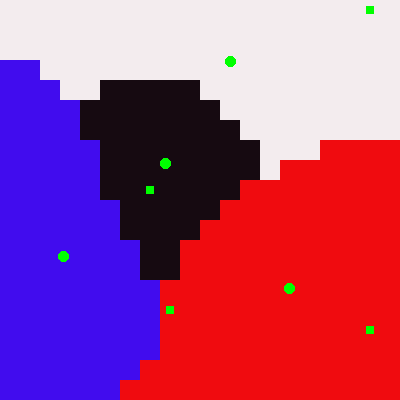
\includegraphics[width=0.4\textwidth]{1a-means}
	\caption{Example of Gaussian means in image 1a}
	\label{fig:1a-means}
\end{figure}
As you can see, the initial guesses were spread out quite evenly and uniformly across the image, and the means converged to points reasonably close to the Euclidean center of each of the colored areas. 
See the appendices for further illustrations.

When the initial guesses were more clumped together or not spread out as widely, results such as in figure \ref{fig:1a-closestart2} could occur, where three of the four Gaussians are bunched together:

\begin{figure}[h]
	\centering
	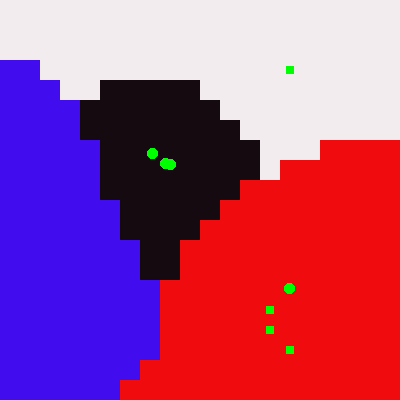
\includegraphics[width=0.4\textwidth]{1a-closestart2}
	\caption{Close starting guesses make for dubious results}
	\label{fig:1a-closestart2}
\end{figure}




\section{Number of clusters}
The most appropriate number of clusters is four for image 1 and five for image 2, and I generally found that using these values yielded the most reasonable results. 
(But see section 3 for why this might not be true for segmentation.)
Using a few more clusters also resulted in mostly sensible results, such as the placements (circles) in figure \ref{fig:2a-6clusters} with six clusters. 

\begin{figure}[h]
	\centering
	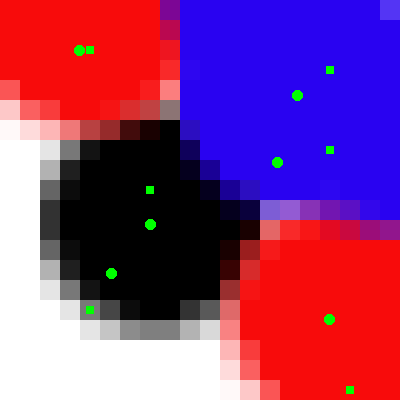
\includegraphics[width=0.4\textwidth]{2a-6clusters}
	\caption{Using more clusters than necessary in image 2a}
	\label{fig:2a-6clusters}
\end{figure}
The Gaussians are placed with means mostly in the center of their ``own'' block of color, with more than one where the block is either too big (as in the blue block in the northwest of figure \ref{fig:2a-6clusters}), or there is more than one block whose mean could be placed in that general area (as in the white and black areas in the southeast).

\begin{figure}[h]
	\centering
	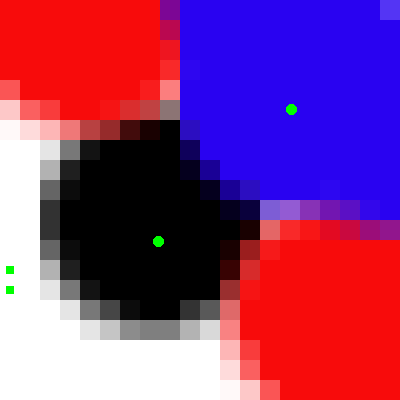
\includegraphics[width=0.4\textwidth]{2a-2clusters}
	\caption{Using fewer clusters than required in image 2a}
	\label{fig:2a-2clusters}
\end{figure}

With images as small as these, it becomes harder to reason about the results when the number of clusters is excessive. 
Using too few clusters, on the other hand, could give both reasonable results, such as in figure \ref{fig:2a-2clusters}, or  confusing and non-obvious placement, such as in figure \ref{fig:1a-2clusters}.

\begin{figure}[h]
	\centering
	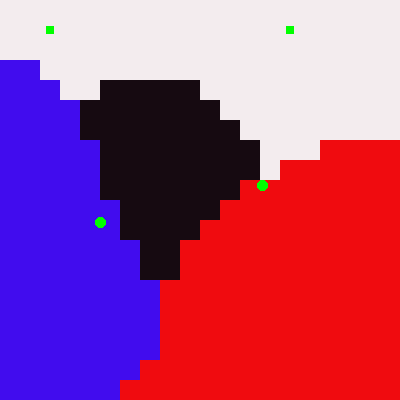
\includegraphics[width=0.4\textwidth]{1a-2clusters}
	\caption{Using fewer clusters than required in image 1a}
	\label{fig:1a-2clusters}
\end{figure}

In general, I would say that the conclusion is pretty intuitive: 
Increasing the number of clusters (within reason) gives accurate results, but with the danger of overfitting the model to the data. 
Using too few clusters gives an inadequate description that does not make much sense and is mostly useless in terms of predictive power.




\section{Segmentation}
A naïve but effective approach to segmentation is to assign each pixel to the color of the closest mean, i.e., the one that minimizes the  distance to that pixel's color and position:
\[
	\mathbf{p} = \arg \min_{\boldsymbol{\mu}} \| \mathbf{x} - \boldsymbol{\mu} \|
\]
Recall that the $\mathbf{x}$ and $\boldsymbol{\mu}$ vectors have components $[r, g, b, x, y]^T$, which means that we minimize over both RGB and Euclidean space. 
This builds on the same idea as the $k$-means algorithm, except that we already know where the means are placed, since the EM algorithm has computed them for us.
Figures \ref{fig:2b-seg} and \ref{fig:2c-seg} provide an example of how this heuristic performs on image 2b and 2c, respectively.

\begin{figure}[h]
	\centering
	
\includegraphics[width=0.4\textwidth]{2b-seg}
	\caption{Naïve segmentation of image 2b, five clusters}
	\label{fig:2b-seg}
\end{figure}

\begin{figure}[h]
	\centering
	
\includegraphics[width=0.4\textwidth]{2c-seg-4clus}
	\caption{Naïve segmentation of image 2c, four clusters}
	\label{fig:2c-seg}
\end{figure}

Observe that in \ref{fig:2b-seg}, the clusters did not each model their own block of color; rather, one of them modeled both of the red areas while one of them modeled the blurry edges between the blocks.
Thus it might turn out that using four clusters may be appropriate for image 2, as evidenced by figure \ref{fig:2c-seg} since giving the edges their own intermediate color as in figure \ref{fig:2b-seg} is arguably a case of overfitting.
Still, using four clusters presents other problems such as in figure \ref{fig:2a-seg2}, where two areas similar in color have been merged together:

\begin{figure}[h]
	\centering
	
\includegraphics[width=0.4\textwidth]{2a-seg2}
	\caption{Segmentation of image 2a with four clusters}
	\label{fig:2a-seg2}
\end{figure}

A more sophisticated segmentation heuristic is to not count all coordinates as equal, but place more weight on one of either the RGB or Euclidean coordinates and less weight on the other. 
Giving more weight to RGB coordinates would tend to put pixels of similar color in the same segment, giving less credence to where they are placed, while giving more weight to the Euclidean coordinates would tend to place pixels that are spatially close together in the same segment.

I have used image 2 in this section, since it is more noisy than image 1 and therefore is more interesting in terms of the difficulty of segmenting it.




\section{Difficulties} 
I was surprised by how little the noise seems to affect segmentation. 
Figure \ref{fig:2c-seg}, for example, is an entirely reasonable segmentation of image 2c, which is filled with noise.
Of course, this assumes that the Gaussian means were placed sensibly in the first place, but I still think the naïve heuristic performed better than expected. 
I think this is a natural attribute of the algorithm itself: 
Since it computes Gaussian averages and then tries to fit the data to the closest mean (in some sense of ``close'') for purposes of segmentation, any variation in the data set is smoothed out to a large extent. 
This is arguably the entire point of segmenting the images at all, namely finding the areas with the most in common and treating them as one.

I will also note that the quality of the segmentation is entirely dependent on the quality of the computed means; if the EM algorithm was initialized badly and the resulting Gaussians were not placed appropriately, the results are useless, as in figures \ref{fig:2a-seg-bad} and \ref{fig:1c-seg-bad}.

\begin{figure}[h]
	\centering
	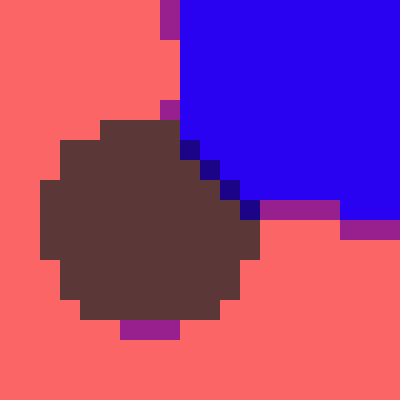
\includegraphics[width=0.4\textwidth]{2a-seg-bad}
	\caption{Botched segmentation of image 2a due to badly placed means: colors are bad and segments are joined}
	\label{fig:2a-seg-bad}
\end{figure}

\begin{figure}[h]
	\centering
	
\includegraphics[width=0.4\textwidth]{1c-seg-bad}
	\caption{Botched segmentation of image 1c due to badly placed means: colors are bad}
	\label{fig:1c-seg-bad}
\end{figure}



\section{Further comments}
\subsection{Page limit}
Since illustrations are not included as part of the page limit, the main part of the text exceeds three pages since I've placed most illustrations inline.
The images clearly take up more than one page, so I hope this is not a problem.

\subsection{Randomization}
I mostly used random initial parameters for the EM algorithm, which meant that it sometimes converged badly and placed the Gaussians in completely inappropriate places.
Setting initial parameters by hand is a possiblility, and though it requires some testing and tweaking to get right, it can produce much more consistently good outcomes.

\subsection{Manual usage}
For the most part, I just ran the script again if the output was a mess or didn't prove the point I was trying to make.
The reader may have to do something similar to recreate the illustrations I have included here, all of which were created with random initialization. 
That is, one should not expect to run the script and get a result that is identical to any illustration presented here.


\appendix

\clearpage
\section{Gaussian means}
With four clusters and random initial means, covariances and weightings, the EM algorithm usually produced results akin to these in image 1:

\begin{figure}[h]
	\centering
	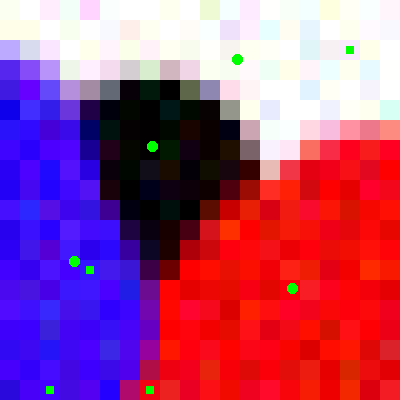
\includegraphics[width=0.35\textwidth]{1b-means}
	\caption{Example of Gaussian means in image 1b}
	\label{fig:1b-means}
\end{figure}

\begin{figure}[h]
	\centering
	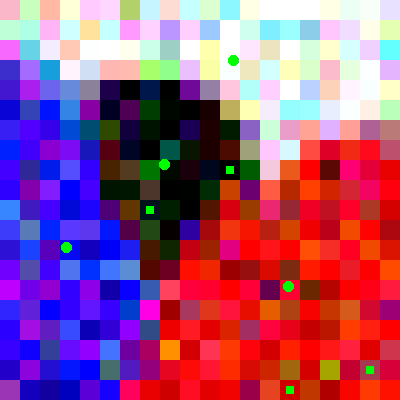
\includegraphics[width=0.35\textwidth]{1c-means}
	\caption{Example of Gaussian means in image 1c}
	\label{fig:1c-means}
\end{figure}

On the other hand, Matlab's EM had a notoriously hard time figuring out image 2; no matter how much noise was present, the white area was rarely assigned its own Gaussian placed squarely in the center of the section.
Results like in figure \ref{fig:2b-means} and \ref{fig:2c-means} were common.
The Gaussian placed on the border of the black and white areas can be considered to generate the elongated white section, then overlaid by a more intense black field that partly covers it.

\begin{figure}[h]
	\centering
	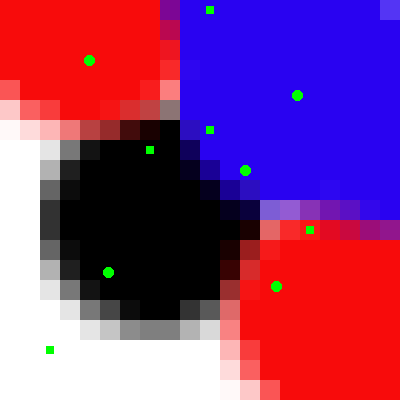
\includegraphics[width=0.35\textwidth]{2a-means}
	\caption{Example of Gaussian means in image 2a}
	\label{fig:2a-means}
\end{figure}

\begin{figure}[h]
	\centering
	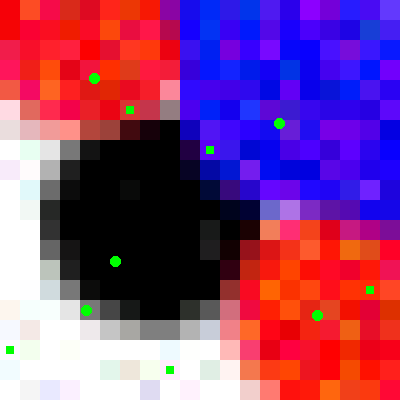
\includegraphics[width=0.35\textwidth]{2b-means}
	\caption{Example of Gaussian means in image 2b}
	\label{fig:2b-means}
\end{figure}

\begin{figure}[h]
	\centering
	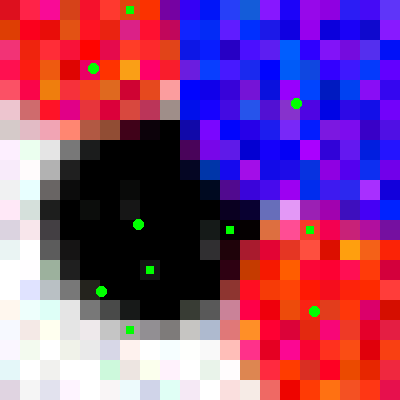
\includegraphics[width=0.35\textwidth]{2c-means}
	\caption{Example of Gaussian means in image 2c}
	\label{fig:2c-means}
\end{figure}



\clearpage
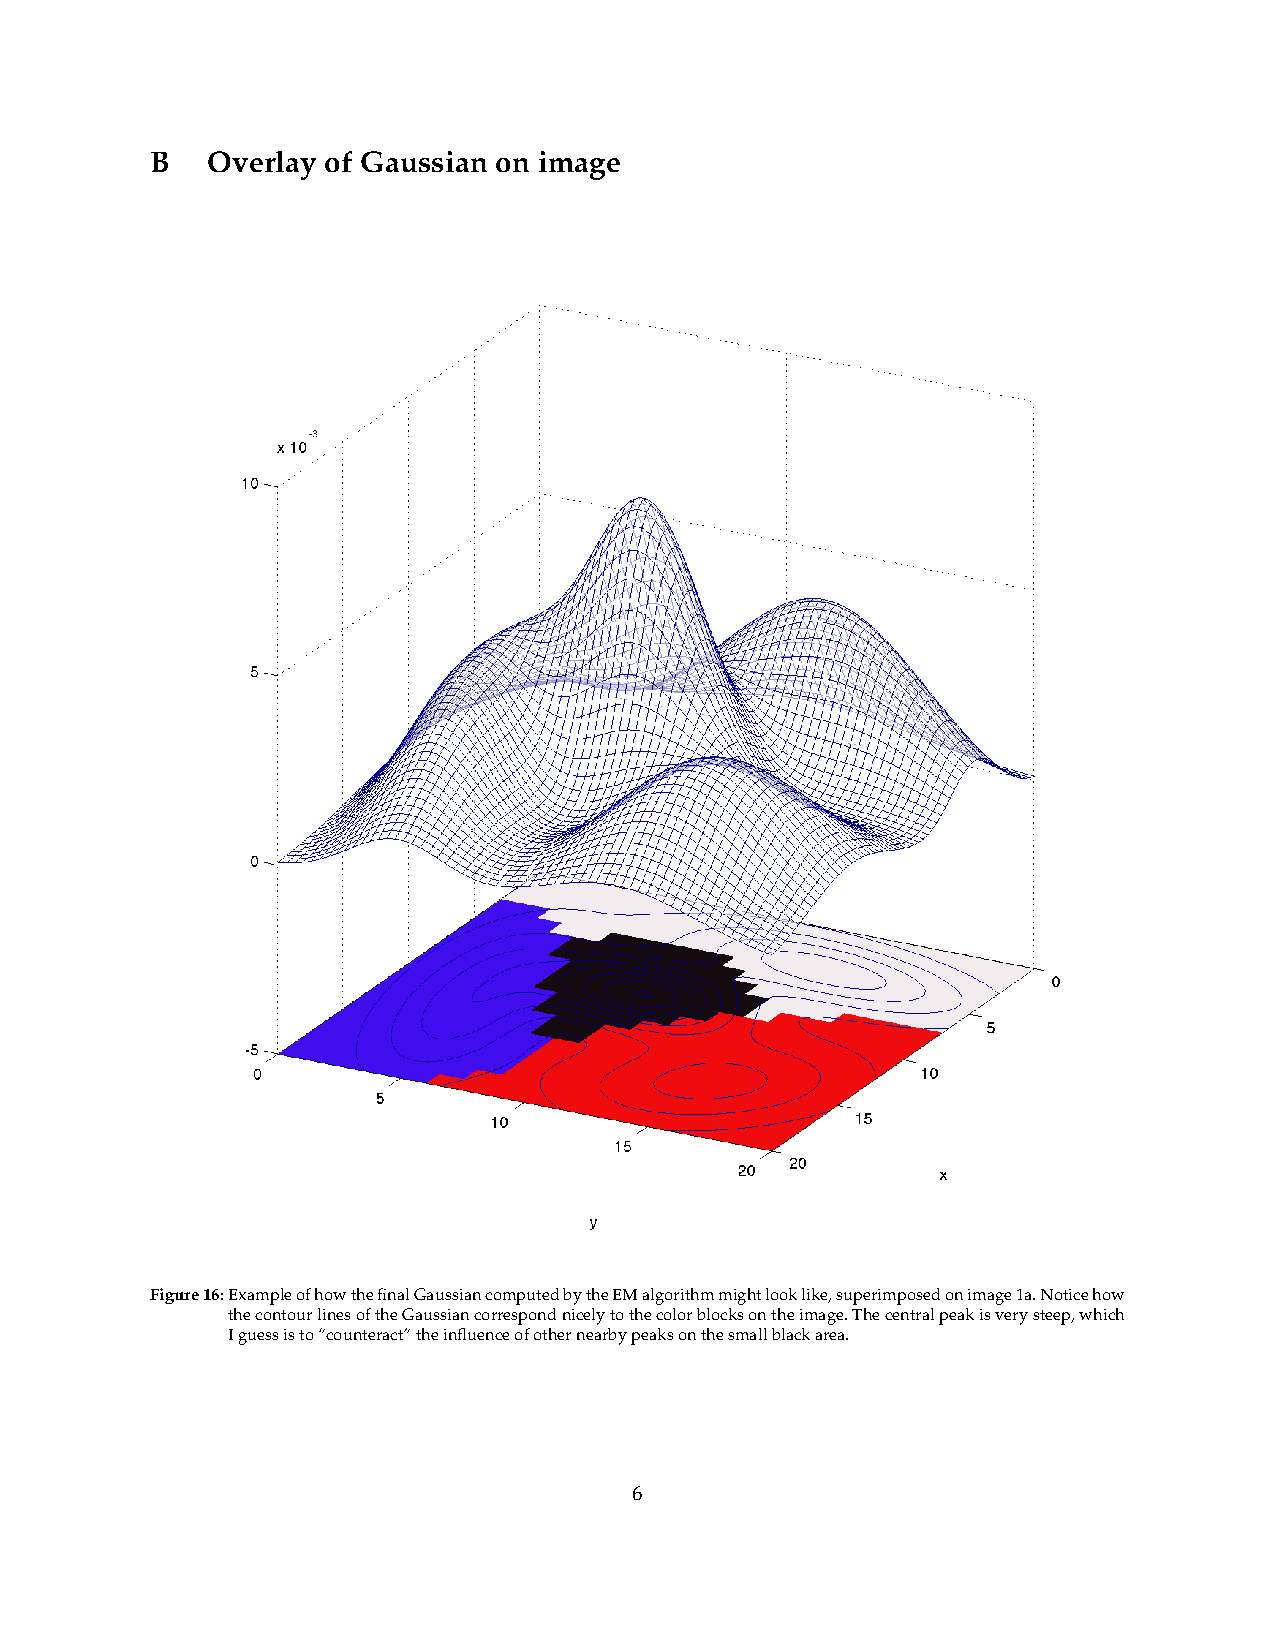
\includepdf{lastpage.pdf}


\end{document}
